\documentclass[../main.tex]{subfiles}

\begin{document}
    \subsection{Planowanie testów.}
    \subsubsection{Szacowanie}
    Szacowanie pozwala na lepszą \textbf{alokację zasobów} i lepszą \textbf{organizację} projektu. Jest podstawą do podjęcia
    decyzji o ograniczeniu zakresu projektu, jeśli estymowany koszt lub czas jest zbyt duży.

    Szacowanie jest \textbf{trudne}. Problemy wynikają nie tylko z samej natury problemu, lecz także z tzw. \textbf{przyczyn politycznych}.

    \textbf{Rola szacowania}
    \begin{itemize}
        \item określenie \textbf{pracochłonności} projektu
        \item określenie \textbf{kosztochłonności} projektu
    \end{itemize}

    Do szacowania można użyć analizy punktów testowcyh (Test Point Analysis) - TMap.

    \subsubsection{Dokumentacja}

    \begin{table}[H]
        \begin{center}
            \begin{tabular}{p{8cm} | p{8cm}}
                \textbf{Cele dokumentowania} & \textbf{Rodzaje dokumentów}\\
                \hline
                \begin{itemize}
                    \item \textbf{opisanie} obowiązujących w organizacji lub projekcie \textbf{reguł, standardów, celów} do osiągnięcia, stanowiących punkt odniesienia podczas prac projektowych
                    \item akceptowanie/zezwalanie/potwierdzanie wykonania określonych czynności
                    \item utrwalenie danych
                    \item pomoc w monitorowaniu i kontroli procesów
                    \item pomoc w opanowaniu złożoności projektów
                    \item mniej lub bardziej formalna \textbf{platforma komunikacji}
                \end{itemize}
                &
                \begin{itemize}
                    \item \textbf{Polityka testów} – wysokopoziomowy opis \textbf{zasad, podejść} i głównych \textbf{zadań} organizacji dotyczących testowania.
                    \item \textbf{Strategia testów} – wysokopoziomowy opis \textbf{poziomów} testów do wykonania oraz testów w ramach tych poziomów dla organizacji lub programu.
                    \item \textbf{Plan testów} – opis \textbf{zakresu, metod, zasobów i harmonogramu} czynności testowych dla projektu.
                    \item \textbf{Dziennik wykonania testów} – zapis czynności testowych.
                \end{itemize}\\
                \hline
            \end{tabular}
        \end{center}
    \end{table}


    \subsubsection{Metryki}
    \begin{table}[H]
        \begin{center}
            \begin{tabular}{p{8cm} p{8cm}}
                \multicolumn{2}{c}{\textbf{ Na podstawie metryk możemy:}}\\
                \begin{itemize}
                    \item \textbf{mierzyć postęp} procesu testowego
                    \item \textbf{obliczyć zwrot} z inwestycji (ROI), tzn. czy proces testowy daje pożądane korzyści
                    \item \textbf{ocenić} i porównać różne możliwe \textbf{podejścia} do testowania
                    \item \textbf{ocenić} i kontrolować \textbf{wydajność} procesu testowego
                \end{itemize}
                &
                \begin{itemize}
                    \item \textbf{ocenić} i kontrolować \textbf{poprawę} procesu testowego
                    \item \textbf{zbudować system „wczesnego ostrzegania”}
                    \item \textbf{zbudować modele predykcyjne}
                    \item porównywać proces z procesami \textbf{konkurencji}
                \end{itemize}\\
            \end{tabular}
        \end{center}
    \end{table}

    \textbf{Wymiary postępu testowania.}
    \begin{itemize}
        \item Ryzyka, defekty, testy i pokrycie – \textbf{metryki ilościowe}
        \item Pewność – najbardziej subiektywna, często \textbf{jakościowa}; pomiar za pomocą ankiet, wywiadów, kwesionariuszy
    \end{itemize}

    \begin{figure}[H]
        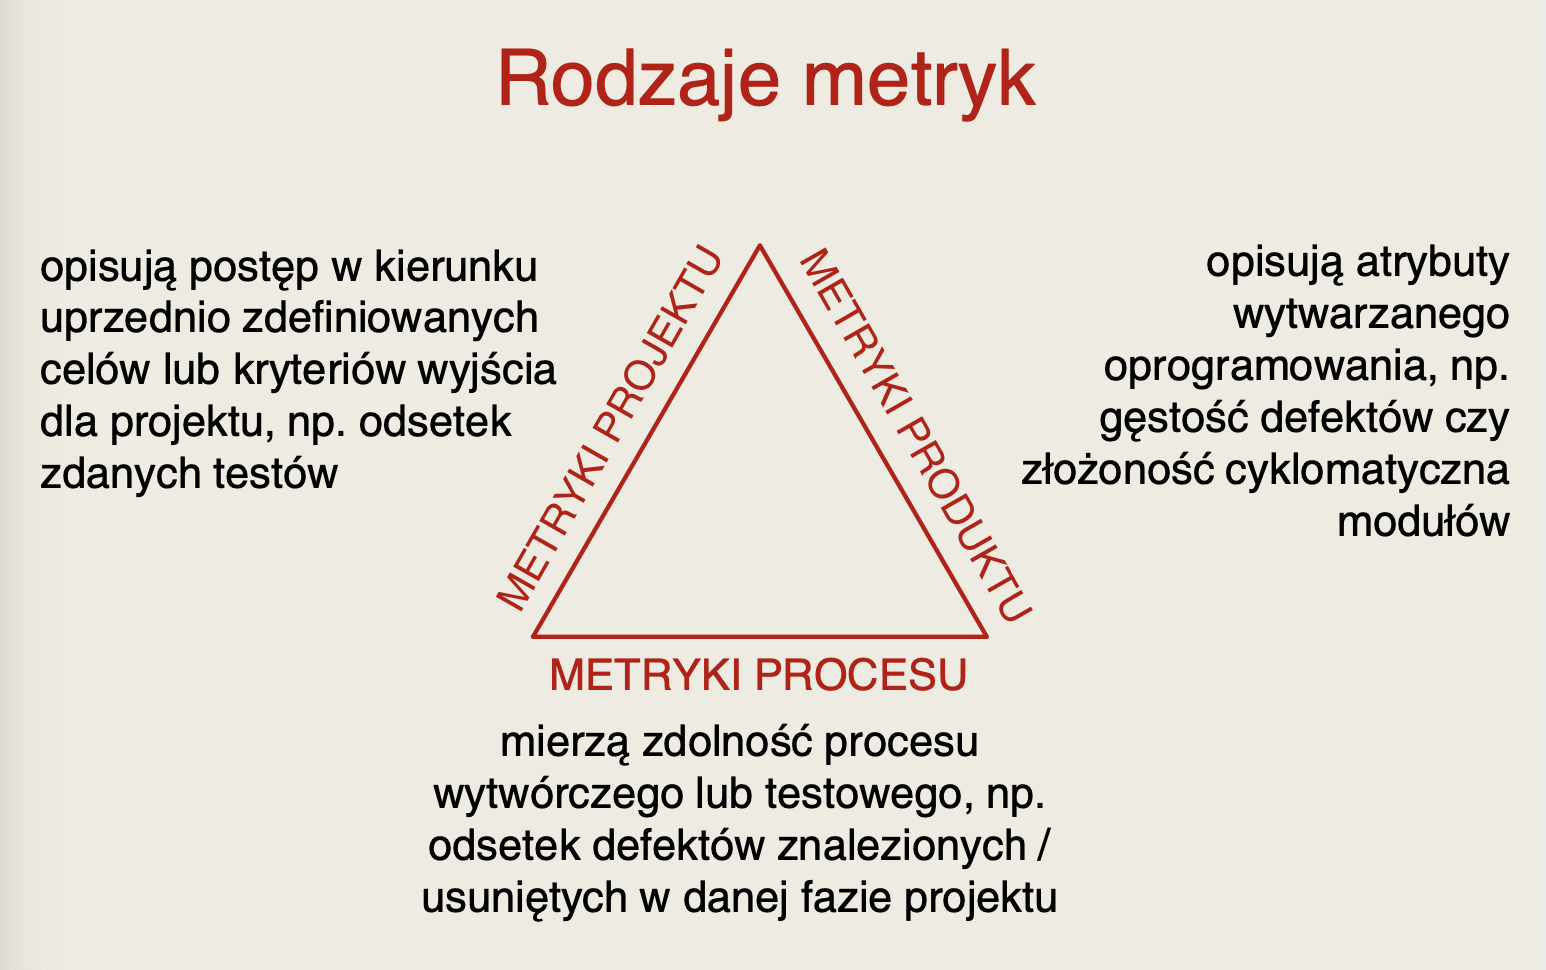
\includegraphics[width=\linewidth]{metryki.png}
    \end{figure}

    $MTTF$ = \textbf{Mean Time To Failure} - średni czas do awarii

    $MTTR$ = \textbf{Mean Time To Repair} - średni czas do naprawy

    $MTBF$ = \textbf{Mean Time Between Failures} - średni czas między awariami

    \begin{table}[H]
        \begin{center}
            \begin{tabular}{p{5cm} p{5cm} p{5cm}}
                \begin{align*}
                    MTTF = \frac{\sum_{i=1}^{N} OK_i}{N}
                \end{align*}
                &
                \begin{align*}
                    MTTR = \frac{\sum_{i=1}^{N} R_i}{N}
                \end{align*}
                &
                \begin{align*}
                    MTBF = MTTF + MTTR
                \end{align*}
            \end{tabular}
        \end{center}
    \end{table}
    Wraz ze wzrostem dojrzałości oprogramowania wzrasta MTTF.

    \textbf{Przykłady metryk}
    \begin{itemize}
        \item Metryki \textbf{ryzyka produktowego} - pokrycie ryzyk
        \item Metryki \textbf{defektów} - MTTF, MTBF, analiza napraw, zgłoszonych defektów
        \item Metryki \textbf{przypadków testowych}
        \item Metryki \textbf{pokrycia} - stopień pokrycia wymagań, kodu, klas równoważności itd.
        \item Metryki \textbf{pewności} - stabilność, niezawodność, ocena klienta
    \end{itemize}

    \subsection{Zarządzanie incydentami}
    \subsubsection{IEEE 1044.}
    Cykl życia defektu wg IEEE 1044.
    \begin{enumerate}
        \item \textbf{Rozpoznanie (recognition)} – zaobserwowanie anomalii (incydent) wskazującej na potencjalny defekt – może nastąpić w dowolnej fazie cyklu życia oprogramowania
        \item \textbf{Badanie (investigation)} – badanie incydentu; może wykryć powiązane problemy i zaproponować rozwiązania
        \item \textbf{Działanie (action)} – możemy chcieć rozwiązać defekt lub podjąć akcje zapobiegania wystąpienia podobnych defektów w przyszłości; po rozwiązaniu muszą nastąpić testy regresji i testy potwierdzające; testy dotychczas blokowane przez defekt mogą zostać wykonane
        \item \textbf{Dyspozycja (disposition)} – zbieranie dalszych informacji i przeniesienie defektu w stan końcowy
    \end{enumerate}

    \begin{figure}[H]
        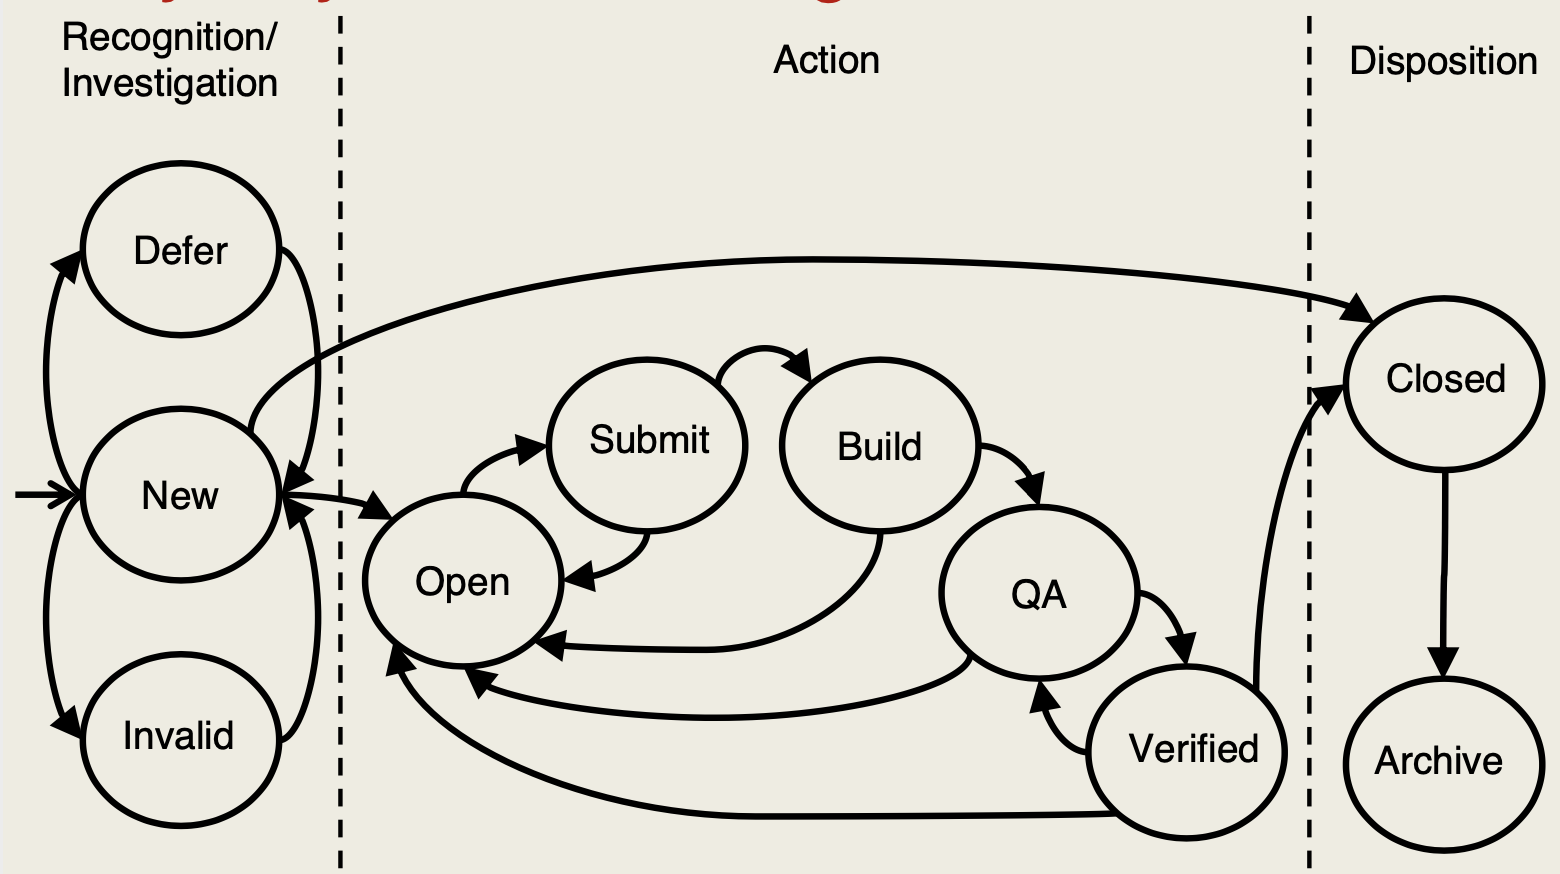
\includegraphics[width=\linewidth]{ieee1044.png}
    \end{figure}


    \begin{table}[H]
        \begin{center}
            \begin{tabular}{ | p{3cm} | p{4cm} | p{4cm} | p{4cm} |}
                \hline
                \multirow{2}{*}{\textbf{Krok}} & \multicolumn{3}{c|}{\textbf{Czynności}}\\
                \cline{2-4}
                \multirow{2}{*}{} & \textbf{rejestruj}\ldots & \textbf{klasyfikuj}\ldots & \textbf{identyfikuj wpływ}\ldots\\
                \hline
                \textbf{Rozpoznanie }& wspomagające informacje
                & na podstawie ważnych atrybutów
                & na podstawie postrzeganego wpływu\\
                \hline
                \textbf{Badanie}
                & zaktualizuj i dodaj dodatkowe informacje
                & zaktualizuj i dodaj klasyfikację na podst. ważnych atrybutów
                & aktualizuj na podstawie badania\\
                \hline
                \textbf{Działanie}
                & dodaj dane oparte o podjęte działanie
                & dodaj dane oparte o podjęte działanie
                & aktualizuj na podstawie działania\\
                \hline
                \textbf{Dyspozycja}
                & dodaj dane bazujące na dyspozycji
                & na podstawie dyspozycji
                & aktualizuj na podstawie dyspozycji\\
                \hline
            \end{tabular}
        \end{center}
    \end{table}


    \begin{table}[H]
        \begin{center}
            \begin{tabular}{| p{8cm} | p{8cm} |}
                \hline
                \textbf{Atrybuty defektu wg IEEE 1044} &   \textbf{Klasyfikacje wpływu defektu wg IEEE 1044}\\
                \hline
                zgłoszenie defektu pozwalające na podjęcie działania jest:
                \begin{itemize}
                    \item \textbf{kompletne} - nie brakuje żadnych ważnych szczegółów,
                    \item \textbf{zwięzłe} - nie zawiera nieistotnych informacji,
                    \item \textbf{precyzyjne} - nie wprowadza czytelnika w błąd,
                    \item \textbf{obiektywne} - bazuje na faktach, nie atakuje nikogo.
                \end{itemize}
                &

                \begin{itemize}
                    \item dotkliwość (severity)
                    \item priorytet
                    \item wartość dla klienta
                    \item sukces misji (mission safety)
                    \item harmonogram projektu
                    \item koszt projektu
                    \item ryzyko projektu
                    \item jakość projektu
                    \item kwestie społeczne
                \end{itemize}\\
                \hline
            \end{tabular}
        \end{center}
    \end{table}

    \subsubsection{Główne modele doskonalenia}
    \begin{table}[H]
        \begin{center}
            \begin{tabular}{p{8cm} p{8cm}}
                \raisebox{-\linewidth}{ 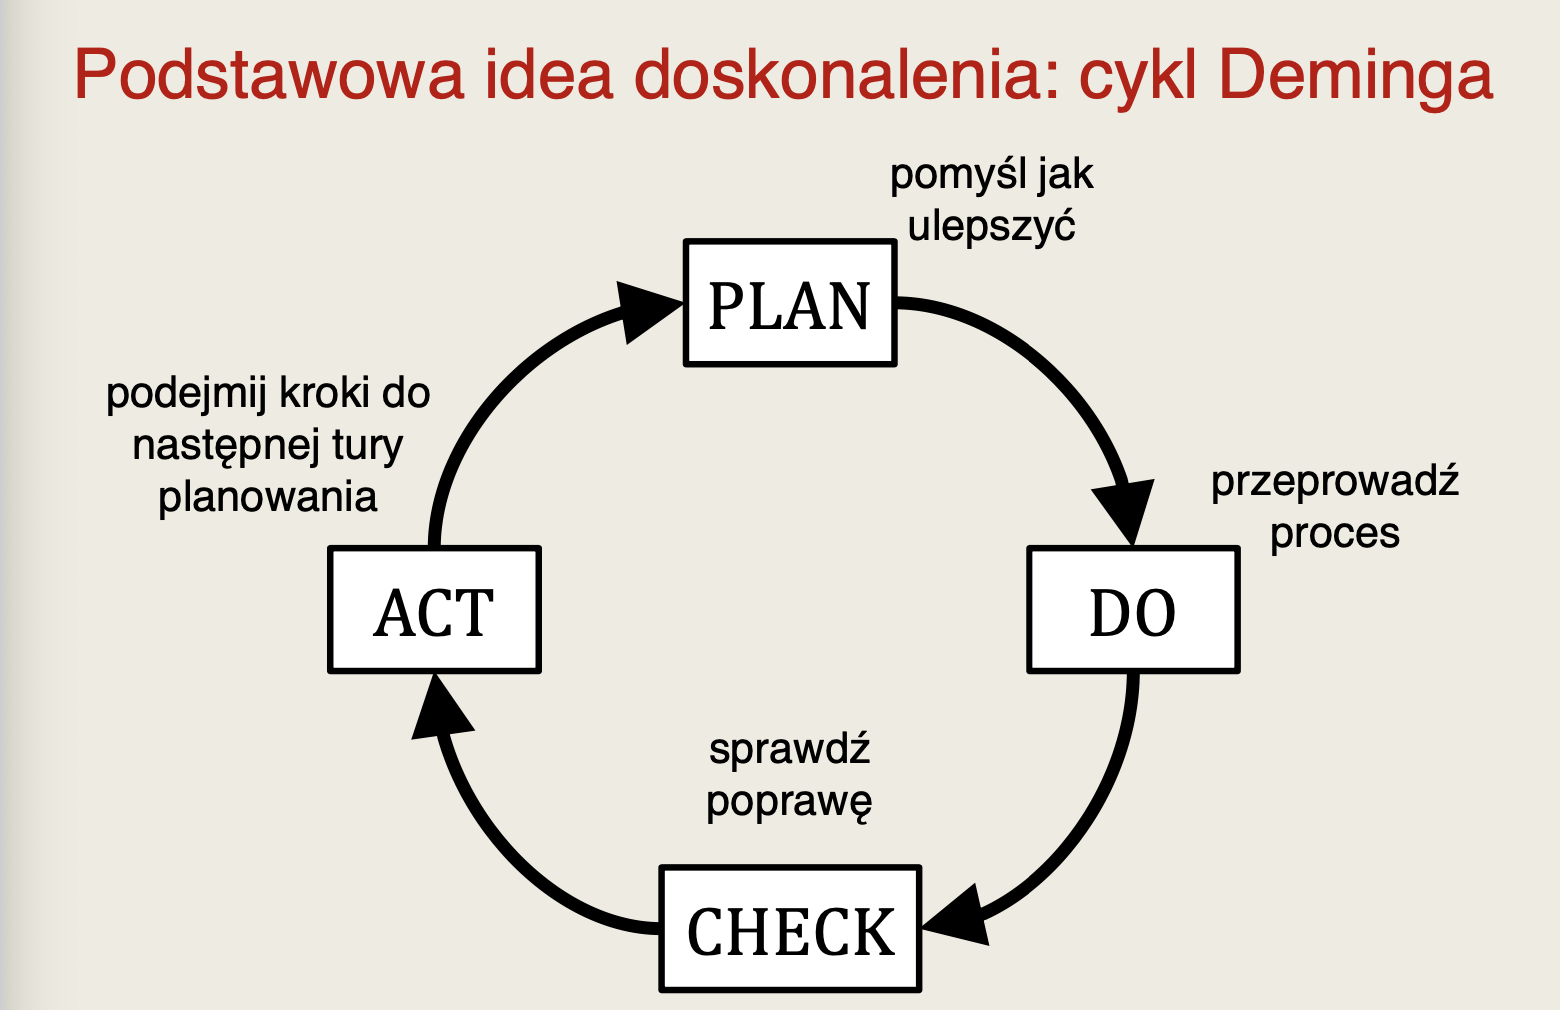
\includegraphics[width=8cm]{deming.png}}
                &
                \begin{itemize}
                    \item Test Maturity Model (TMM)
                    \item Test Process Improvement (TPI, TPI Next)
                \end{itemize}
                \begin{itemize}
                    \item Critical Testing Processes (CTP)
                    \item Systematic Test and Evaluation Process (STEP)
                    \item Test Organization Maturity (TOM)
                    \item Test Improvement Model (TIM)
                    \item Software Quality Rank (SQR)
                    \item TMap
                \end{itemize}\\
            \end{tabular}
        \end{center}
    \end{table}

    \textbf{Modele referencyjne}
    \begin{itemize}
        \item \textbf{procesu}
        \begin{itemize}
            \item (jednowymiarowa) ocena dojrzałości procesu
            \item wskazują kolejność usprawnień
        \end{itemize}
        \item \textbf{zawartości}
        \begin{itemize}
            \item opisują ważne procesy software’owe i co powinno się z nimi robić
            \item ale nie szeregują zadań w żadnej kolejności
        \end{itemize}
    \end{itemize}
\end{document}